\documentclass[]{beamer}
\usepackage[T1]{fontenc}
\usepackage[utf8]{inputenc}
\usepackage{lmodern}
\usepackage[italian]{babel}

\title{Il secondo principio della termodinamica}
\author{\texorpdfstring{Mattia Cozzi\newline\href{mailto:cozzimattia@gmail.com}{\texttt{cozzimattia@gmail.com}}}{Mattia Cozzi}}
\date{a.s.~2023/2024}

%\documentclass[handout]{beamer}     %usare questa classe per generare l'handout
%\usepackage{pgfpages}   %per mostrare più quadri nella stessa pagina
%\pgfpagesuselayout{4 on 1}[a4paper,border shrink=5mm,landscape]
\usetheme{Singapore}
%\useoutertheme[left]{sidebar} %elementi intorno alle diapositive
\setbeamercovered{dynamic} %modifica l'aspetto del testo grigetto delle diapositive future. Argomenti: invisible/transparent/dynamic
\usecolortheme{orchid}
%COLORE PRINCIPALE
\definecolor{marroncino}{RGB}{156, 26, 0} % UBC Blue (primary)
\setbeamercolor{structure}{fg=marroncino} % itemize, enumerate, etc

\theoremstyle{plain}
\newtheorem{teorema}{Teorema}

\usepackage{tikz}


\usepackage{pgf,pgfplots,graphicx}
\usetikzlibrary{angles,quotes,arrows,shapes,decorations.markings}
\pgfplotsset{compat=1.15}
\usepgfplotslibrary{units,fillbetween} % to add units easily to axis
\tikzset{fleche/.style args={#1:#2}{postaction=decorate,decoration={name=markings,mark=at position #1 with {\arrow[#2,scale=2]{>}}},},}



\begin{document}

\begin{frame}
  \titlepage
\end{frame}





\begin{frame}
\frametitle{Contenuti}
\tableofcontents
\end{frame}


%mancano degli esempi, soprattutto sul ciclo di carnot

\section{Macchine termiche}

\begin{frame}
\frametitle{Contesto storico}
\begin{columns}
\begin{column}{0.2\textwidth}
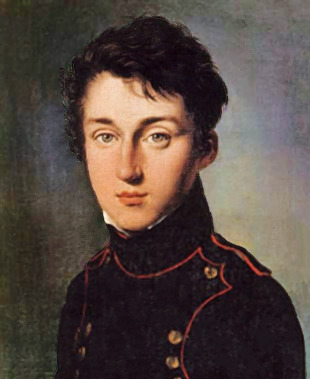
\includegraphics[width=\columnwidth]{img/carnot.jpg}
\end{column}
\begin{column}{0.7\textwidth}
1824\\Sadi Carnot pubblica le \emph{Riflessioni sulla potenza motrice del fuoco}, testo che contiene la sua teoria sulle macchine termiche.\pause

\begin{itemize}
\item<2-> I motori a vapore sono utilizzati su vasta scala (macchina di Watt, 1765);
\item<3-> Il principio di conservazione dell'energia non è ancora stato enunciato;
\item<4-> Non è stata dimostrata l'equivalenza tra calore e lavoro (Joule, 1847);
\item<5-> Il modello per lo studio del calore è la \emph{teoria del calorico} (un ipotetico fluido che passa da un corpo ad un altro).
\end{itemize}
\end{column}
\end{columns}
\end{frame}

\begin{frame}
\frametitle{Definizione}
\begin{block}{Macchina termica}
Una macchina termica è un dispositivo che:\pause
\begin{itemize}
  \item assorbe energia sotto forma di \emph{calore};\pause
  \item restituisce energia sotto forma di \emph{lavoro};\pause
  \item agisce mediante una o più \emph{trasformazioni cicliche}.
\end{itemize}
\end{block}
\end{frame}

\begin{frame}
\frametitle{Centrale termoelettrica}
  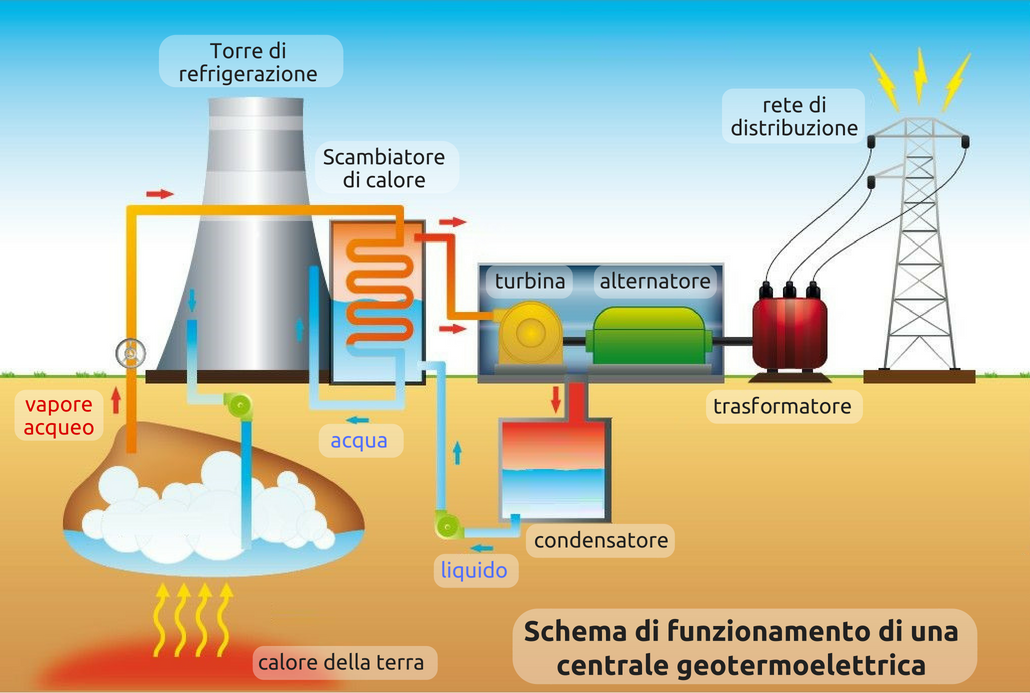
\includegraphics[width=\columnwidth]{img/centraletermoelettrica.png}
\end{frame}


\begin{frame}
\frametitle{La macchina termica ideale}
  Immaginiamo di lavorare con una \alert{macchina termica ideale}, ovvero un cilindro pieno di gas ideale, dotato di un pistone mobile.\pause
  
  ~
  
  Tale macchina ideale:\pause
  \begin{itemize}
    \item riceve una quantità di calore $ Q_2 $ da una \emph{sorgente calda} a temperatura $ T_2 $; ricevendo calore, \colorbox{marroncino!30}{$ Q_2 > 0 $};\pause
    \item cede una quantità di calore $ Q_1 $ ad una \emph{sorgente fredda} a temperatura $ T_1 < T_2 $; cedendo calore, \colorbox{marroncino!30}{$ Q_1 < 0 $}.
  \end{itemize}
\end{frame}


\begin{frame}
\frametitle{Schema della macchina ideale}
\begin{figure}\centering
\begin{tikzpicture}[scale=0.5]

\draw (0,0) -- (5,0);
\draw [fill=orange] (.8,0) rectangle (1,4);
\draw [fill=orange] (4,0) rectangle (4.2,4);
\draw [fill=black] (1,1) rectangle (4,1.1);
\node [below] at (2.5,5) {stato A};

\pause

\draw (6,0) -- (11,0);
\draw [fill=black!30,black!30] (7,2.33) rectangle (10,2.43);
\draw [fill=black!20,black!20] (7,1.66) rectangle (10,1.76);
\draw [fill=black!10,black!10] (7,1) rectangle (10,1.1);
\draw [fill=orange] (6.8,0) rectangle (7,4);
\draw [fill=orange] (10,0) rectangle (10.2,4);
\draw [fill=black] (7,3) rectangle (10,3.1);
\node [below] at (8.5,5) {stato B};
\draw [->,thick,red] (8.5,-.4) -- (8.5,1);
\node [right,red] at (8.5,.6) {$ Q_2 $};
\node [below,red] at (8.5,-.2) {sorgente calda};

\pause

\draw (12,0) -- (17,0);
\draw [fill=black!10,black!10] (13,3) rectangle (16,3.1);
\draw [fill=black!20,black!20] (13,2.33) rectangle (16,2.43);
\draw [fill=black!30,black!30] (13,1.66) rectangle (16,1.73);
\draw [fill=orange] (12.8,0) rectangle (13,4);
\draw [fill=orange] (16,0) rectangle (16.2,4);
\draw [fill=black] (13,1) rectangle (16,1.1);
\node [below] at (14.5,5) {stato A};
\draw [->,thick,blue] (14.5,.8) -- (14.5,-.4);
\node [right,blue] at (14.5,.5) {$ Q_1 $};
\node [below,blue] at (14.5,-.2) {sorgente fredda};
\end{tikzpicture}
\end{figure}
\end{frame}

\begin{frame}
  \frametitle{Bilancio energetico}
  Le trasformazioni in una macchina ideale sono tutte cicliche e ideali; la variazione di energia interna del sistema sarà nulla, e quindi:
  \[ \Delta U = Q - L = 0 \,\,(PPT)\qquad\Longrightarrow\qquad L = Q \]\pause

  ~
  
  Poiché $ Q $ indica il \emph{calore totale scambiato} durante la trasformazione, cioè la somma di $ Q_2 $ (positivo) e $ Q_1 $ (negativo), vale:
    \begin{center}
\colorbox{marroncino!30}{$ L = Q_2 + Q_1 = Q_2 - |Q_1| $}
\end{center}\pause
  L'equazione precedente ci dice che \alert{non tutto il calore assorbito dalla macchina viene trasformato in lavoro}!
\end{frame}



\begin{frame}
\frametitle{Schema di una macchina termica}
\begin{figure}
\begin{tikzpicture}[scale=0.5]
\node [above,purple] at (0,2) {M};
\draw [purple, ultra thick] (0,0) circle [radius=2];
\draw (-4,2) -- (-4,-2);
\draw (-4,2) -- (-5.5,2);
\draw (-4,-2) -- (-5.5,-2);
\node [left,red] at (-4,0) {$ T_2 $};

\draw (4,2) -- (4,-2);
\draw (4,2) -- (5.5,2);
\draw (4,-2) -- (5.5,-2);
\node [right,blue] at (4,0) {$ T_1 $};

\pause

\draw [->,thick,red] (-4,0) -- (-2,0);
\node [below,red] at (-3,0) {$ Q_2 $};

\pause

\draw [->,thick,blue] (2,0) -- (4,0);
\node [below,blue] at (3,0) {$ Q_1 $};

\draw [->,thick] (0,-2) -- (0,-4);
\node [right] at (0,-3) {$ L $};
\end{tikzpicture}
\end{figure}
\end{frame}

\begin{frame}
\frametitle{Esercizi}
\begin{exampleblock}{Lavoro compiuto da una macchina}
  \small{
  Una macchina termica compie $ 1,20 \times 10^{6} $ cicli completi, assorbendo dalla sorgente calda una quantità di energia pari a $ 5,60 \times 10^{7} \, J $. In ogni ciclo essa cede alla sorgente fredda una quantità di calore pari $ 31,8 \, J $.

  Qual è la quantità totale di lavoro compiuta dalla macchina?\hspace*{\fill}[$ 1,79 \times 10^{7} \, J $]}
\end{exampleblock}

~

\begin{exampleblock}{Calore assorbito}
  \small{
  Una macchina termica cede alla sorgente fredda una quantità di calore che permette di elevare la temperatura di una massa di $ 100 \, kg $ di acqua da $ 20,0 \, ^\circ C $ a $ 30,0 \, ^\circ C $ e produce un lavoro di $ 3,20 \times 10^{6} \, J $.

  Calcola la quantità di calore assorbita dalla sorgente calda.\hspace*{\fill}[$ 7,39 \times 10^{6} \, J $]}
\end{exampleblock}
\end{frame}


\section{Enunciati}

\begin{frame}
  \frametitle{L'enunciato di Kelvin}
  A Lord Kelvin dobbiamo una delle \emph{versioni} del \alert{secondo principio della termodinamica}.
  
  ~
  
  \begin{block}{Enunciato di Kelvin (1851)}
    È impossibile realizzare una trasformazione il cui \emph{unico} risultato sia quello di assorbire una determinata quantità di calore da un’\emph{unica} sorgente e trasformarla \emph{integralmente} in lavoro.
  \end{block}
  \end{frame}
  


\begin{frame}
\frametitle{Trasformazioni impossibili e trasformazioni possibili}
\begin{columns}
\begin{column}{0.4\textwidth}
Proibita da Lord Kelvin
\begin{figure}\centering
\begin{tikzpicture}[scale=0.35]
\node [above,purple] at (0,2) {M};
\draw [purple, ultra thick] (0,0) circle [radius=2];
\draw (-4,2) -- (-4,-2);
\draw (-4,2) -- (-5.5,2);
\draw (-4,-2) -- (-5.5,-2);
\node [left,red] at (-4,0) {$ T_2 $};

\draw (4,2) -- (4,-2);
\draw (4,2) -- (5.5,2);
\draw (4,-2) -- (5.5,-2);
\node [right,blue] at (4,0) {$ T_1 $};

\draw [->,thick,red] (-4,0) -- (-2,0);
\node [below,red] at (-3,0) {$ Q $};

\draw [->,thick] (0,-2) -- (0,-4);
\node [right] at (0,-3) {$ L $};
\end{tikzpicture}
\end{figure}
\[ L=Q \]
\end{column}\pause
\begin{column}{0.4\textwidth}
Consentita da Lord Kelvin
\begin{figure}\centering
\begin{tikzpicture}[scale=0.35]
\node [above,purple] at (0,2) {M};
\draw [purple, ultra thick] (0,0) circle [radius=2];
\draw (-4,2) -- (-4,-2);
\draw (-4,2) -- (-5.5,2);
\draw (-4,-2) -- (-5.5,-2);
\node [left,red] at (-4,0) {$ T_2 $};

\draw (4,2) -- (4,-2);
\draw (4,2) -- (5.5,2);
\draw (4,-2) -- (5.5,-2);
\node [right,blue] at (4,0) {$ T_1 $};

\draw [->,thick,red] (-4,0) -- (-2,0);
\node [below,red] at (-3,0) {$ Q_2 $};

\draw [->,thick,blue] (2,0) -- (4,0);
\node [below,blue] at (3,0) {$ Q_1 $};

\draw [->,thick] (0,-2) -- (0,-4);
\node [right] at (0,-3) {$ L $};
\end{tikzpicture}
\end{figure}
\[ L < Q_2 \]
\end{column}
\end{columns}
\end{frame}

\begin{frame}
  \frametitle{L'enunciato di Clausius}
  Una formulazione alternativa del \alert{secondo principio della termodinamica} si deve a Rudolf Clausius.
  
  ~
  
  \begin{block}{Enunciato di Clausius (1854)}
    È impossibile realizzare una trasformazione il cui \emph{unico} risultato sia quello di fare passare calore da un corpo più freddo a uno più caldo.
  \end{block}
  \end{frame}
  

\begin{frame}
\frametitle{Quanti ``secondi principi della termodinamica'' ci sono?}
\pause
\alert<2>{Uno solo}, che può essere espresso con uno qualunque tra i due enunciati.
\pause

~

I due enunciati sono infatti \alert{logicamente equivalenti}:
\begin{center}
Kelvin \emph{sse} Clausius
\end{center}
\begin{figure}\centering
\begin{tabular}{|c|c|c|}\hline
  A&B&A \emph{sse} B\\\hline
  V&V&V \\\hline
  V&F&F \\\hline
  F&V&F \\\hline
  F&F&V \\\hline
\end{tabular}
\end{figure}

\end{frame}

  

\section{Rendimento}

\section{Rendimento}

\begin{frame}
  \frametitle{Rendimento di una macchina termica (1)}
  \begin{block}{Definizione di rendimento}
    \begin{center}
      \colorbox{marroncino!30}{$ \eta = \dfrac{L}{Q_2} $}
    \end{center}\pause
\end{block}

~

\begin{alertblock}{Significato del rendimento}
  Il rendimento (numero puro) è una percentuale. Se $ \eta = 0,42 $, allora il $ 42\% $ del calore assorbito viene tramutato in lavoro.
\end{alertblock}
\end{frame}

\begin{frame}
  \frametitle{L'enunciato del rendimento}
  Possiamo ora dare una nuova versione del \alert{secondo principio della termodinamica}, anch'essa logicamente equivalente alle altre.
  
  ~
    \begin{block}{Enunciato del rendimento}
      È impossibile progettare una macchina termica che abbia rendimento uguale a 1, cioè che trasformi \emph{interamente} il calore assorbito in lavoro.
    \end{block}
  \end{frame}
  

\begin{frame}
  \frametitle{Rendimento di alcuni dispositivi (1)}
  \begin{columns}
    \begin{column}{0.3\textwidth}
      \begin{figure}
        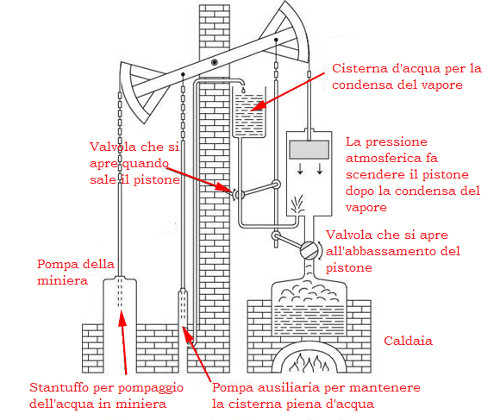
\includegraphics[width=\columnwidth]{img/newcomen.jpg}
      \end{figure}
      Macchina di Newcomen (1712)
      
      $ \eta = 0,007 = 0,7 \% $
    \end{column}
    \begin{column}{0.3\textwidth}
      \visible<2-3>{\begin{figure}
        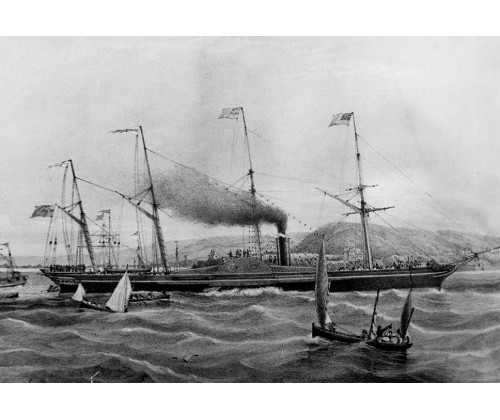
\includegraphics[width=\columnwidth]{img/greatwestern.jpg}
      \end{figure}
      Great Western (1837)
      
      $ \eta = 0,03 = 3 \% $}
    \end{column}
    \begin{column}{0.3\textwidth}
      \visible<3>{\begin{figure}
        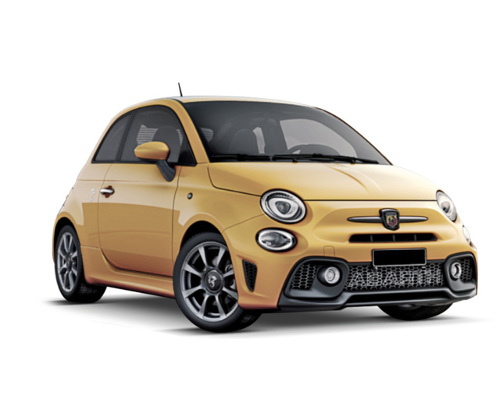
\includegraphics[width=\columnwidth]{img/benzina.jpg}
      \end{figure}
      Motore a benzina (recente)
      
      $ \eta = 0,25 = 25 \% $}
    \end{column}

  \end{columns}
\end{frame}


\begin{frame}
  \frametitle{Rendimento di alcuni dispositivi (2)}
  \begin{columns}
    \begin{column}{0.3\textwidth}
      \begin{figure}
        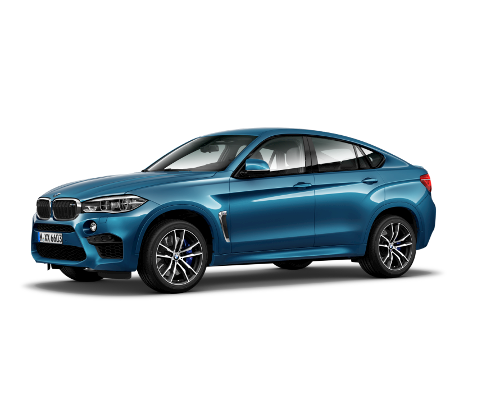
\includegraphics[width=\columnwidth]{img/diesel.png}
      \end{figure}
      Motore diesel (recente)
      
      $ \eta = 0,40 = 40 \% $
    \end{column}
    \begin{column}{0.3\textwidth}
      \visible<2-3>{\begin{figure}
        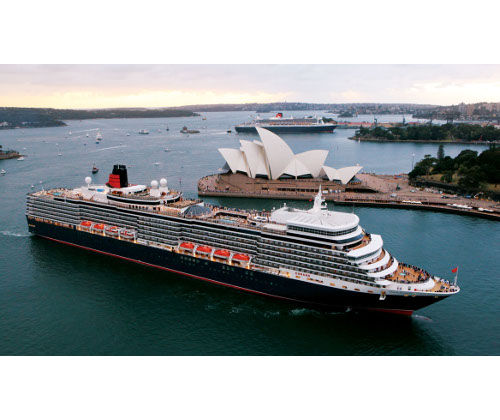
\includegraphics[width=\columnwidth]{img/queenmary2.jpg}
      \end{figure}
      Queen Mary 2 (2003)
      
      $ \eta = 0,44 = 44 \% $}
    \end{column}
    \begin{column}{0.3\textwidth}
      \visible<3>{\begin{figure}
        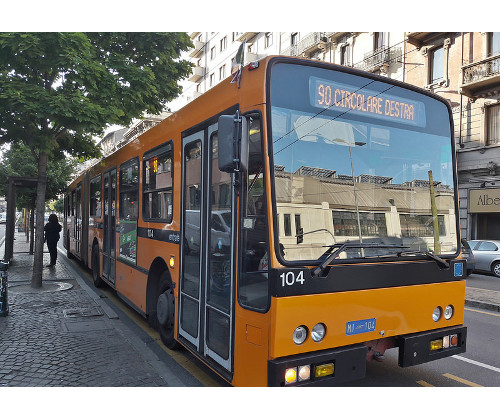
\includegraphics[width=\columnwidth]{img/90.jpg}
      \end{figure}
      Circolare destra (1951)
      
      $ \eta = 0,90 = 90 \% $}
    \end{column}
  \end{columns}

  ~

  ~

  \visible<3>{Notiamo tuttavia che la circolare destra non è una macchina termica: usa infatti un \emph{motore elettrico}.}
\end{frame}

\begin{frame}
  \frametitle{Esercizi}
  \begin{exampleblock}{Calore assorbito}
    \small{
    Una locomotiva a calore dell'Ottocento aveva all'incirca un rendimento dell'$ 8\% $.
  
    Per ottenere un lavoro utile pari a $ 400 \, kJ $, quanto calore si doveva assorbire dalla caldaia?\hspace*{\fill}[$ 5 \, MJ $]}
  \end{exampleblock}
  
  ~
  
  \begin{exampleblock}{Calcolo del rendimento}
    \small{
    Una macchina termica eroga una potenza di $ 3,40 \times 10^{3} \, W $ e il calore emesso durante il ciclo termodinamico in un'ora riscalda una massa di $ 200 \, kg $ d'acqua portando la sua temperatura da $ 20 \, ^\circ C $ a $ 32 \, ^\circ C $.
  
    Qual è il rendimento della macchina?\hspace*{\fill}[$ 0,55 $]}
  \end{exampleblock}
  \end{frame}
\end{document}
